\documentclass[11pt,A4paper,]{article}
\usepackage{lmodern}
\usepackage{amssymb,amsmath}
\usepackage{ifxetex,ifluatex}
\usepackage{fixltx2e} % provides \textsubscript
\ifnum 0\ifxetex 1\fi\ifluatex 1\fi=0 % if pdftex
  \usepackage[T1]{fontenc}
  \usepackage[utf8]{inputenc}
\else % if luatex or xelatex
  \ifxetex
    \usepackage{mathspec}
  \else
    \usepackage{fontspec}
  \fi
  \defaultfontfeatures{Ligatures=TeX,Scale=MatchLowercase}
    \setmainfont[Numbers=Lining]{Brill}
\fi
% use upquote if available, for straight quotes in verbatim environments
\IfFileExists{upquote.sty}{\usepackage{upquote}}{}
% use microtype if available
\IfFileExists{microtype.sty}{%
\usepackage{microtype}
\UseMicrotypeSet[protrusion]{basicmath} % disable protrusion for tt fonts
}{}
\usepackage[margin=1in]{geometry}
\usepackage{hyperref}
\hypersetup{unicode=true,
            pdftitle={A time-aligned account of lingual and laryngeal gestures using ultrasound tongue imaging (UTI) and electroglottography (EGG)},
            pdfauthor={Stefano Coretta},
            pdfborder={0 0 0},
            breaklinks=true}
\urlstyle{same}  % don't use monospace font for urls
\usepackage{natbib}
\bibliographystyle{unified.bst}
\usepackage{longtable,booktabs}
\usepackage{graphicx,grffile}
\makeatletter
\def\maxwidth{\ifdim\Gin@nat@width>\linewidth\linewidth\else\Gin@nat@width\fi}
\def\maxheight{\ifdim\Gin@nat@height>\textheight\textheight\else\Gin@nat@height\fi}
\makeatother
% Scale images if necessary, so that they will not overflow the page
% margins by default, and it is still possible to overwrite the defaults
% using explicit options in \includegraphics[width, height, ...]{}
\setkeys{Gin}{width=\maxwidth,height=\maxheight,keepaspectratio}
\IfFileExists{parskip.sty}{%
\usepackage{parskip}
}{% else
\setlength{\parindent}{0pt}
\setlength{\parskip}{6pt plus 2pt minus 1pt}
}
\setlength{\emergencystretch}{3em}  % prevent overfull lines
\providecommand{\tightlist}{%
  \setlength{\itemsep}{0pt}\setlength{\parskip}{0pt}}
\setcounter{secnumdepth}{5}
% Redefines (sub)paragraphs to behave more like sections
\ifx\paragraph\undefined\else
\let\oldparagraph\paragraph
\renewcommand{\paragraph}[1]{\oldparagraph{#1}\mbox{}}
\fi
\ifx\subparagraph\undefined\else
\let\oldsubparagraph\subparagraph
\renewcommand{\subparagraph}[1]{\oldsubparagraph{#1}\mbox{}}
\fi

%%% Use protect on footnotes to avoid problems with footnotes in titles
\let\rmarkdownfootnote\footnote%
\def\footnote{\protect\rmarkdownfootnote}

%%% Change title format to be more compact
\usepackage{titling}

% Create subtitle command for use in maketitle
\newcommand{\subtitle}[1]{
  \posttitle{
    \begin{center}\large#1\end{center}
    }
}

\setlength{\droptitle}{-2em}
  \title{A time-aligned account of lingual and laryngeal gestures using
ultrasound tongue imaging (UTI) and electroglottography (EGG)}
  \pretitle{\vspace{\droptitle}\centering\huge}
  \posttitle{\par}
  \author{Stefano Coretta}
  \preauthor{\centering\large\emph}
  \postauthor{\par}
  \predate{\centering\large\emph}
  \postdate{\par}
  \date{14/01/2017}

\usepackage{cleveref}

\begin{document}
\maketitle

{
\setcounter{tocdepth}{2}
\tableofcontents
}
\section{Introduction}\label{introduction}

This document

\section{Purpose}\label{purpose}

The combination of techniques described in the following sections allows
a synchronous mapping of lingual gestures and phonation during speech.
Such methodology enables a time-aligned account of the movements of the
tongue and the concomitant configuration of the glottis that
characterises phonation. These techniques employ ultrasound tongue
imaging (UTI) and electroglottography (EGG) for the simultaneous
acquisition of articulatory data from, respectively, the oral cavity and
the glottis.

\subsection{Ultrasound tongue imaging}\label{ultrasound-tongue-imaging}

Ultrasound tongue imaging (UTI) uses ultrasonography for charting the
movements of the tongue into a two-dimensional image. In medical
sonography, ultrasound waves (sound waves at high frequencies, ranging
between 2 and 14 MHz) are emitted from a probe in a fan-like manner, and
travel through organic tissue (such as skin and muscles). When the
surface of a material with different density is hit, the ultrasound
waves are partially reflected, and such ``echo'' is registered by the
probe. These echoes can then be plotted on a two-dimensional graph,
where different densities are represented by different shades (higher
densities are brighter, while lower densities are darker). The graph, or
ultrasound image, will show high density surfaces as very bright lines,
surrounded by darker areas. By positioning the ultrasound probe in
contact with the submental triangle (the surface below the chin),
sagittally oriented, it is possible to infer the cross-sectional profile
of the tongue, which appears as a bright line in the resulting
ultrasound image.

\subsection{Electroglottography}\label{electroglottography}

Electroglottography \citep{fabre1957} is a technique that measures the
size of contact between the vocal folds (the Vocal Folds Contact Area,
VFCA). A high frequency low voltage electrical current is sent through
two electrodes which are in contact with the surface of the neck, one on
each side of the thyroid cartilage (\Cref{f:egg-setup}). The impedance
of the current is directly correlated with VFCA, while its amplitude is
inversely correlated. Thus, impedance increases with lower VFCA and
decreases with higher VFCA. Conversely, amplitude decreases when the
VFCA increases and it increases when the VFCA decreases. The EGG unit
registers changes in impedance and it converts it in amplitude. Its
output is a synchronised stereo recording which contains the EGG signal
from the electrodes in right channel and the audio signal from the
microphone in the left channel.

\begin{figure}[htbp]
\centering
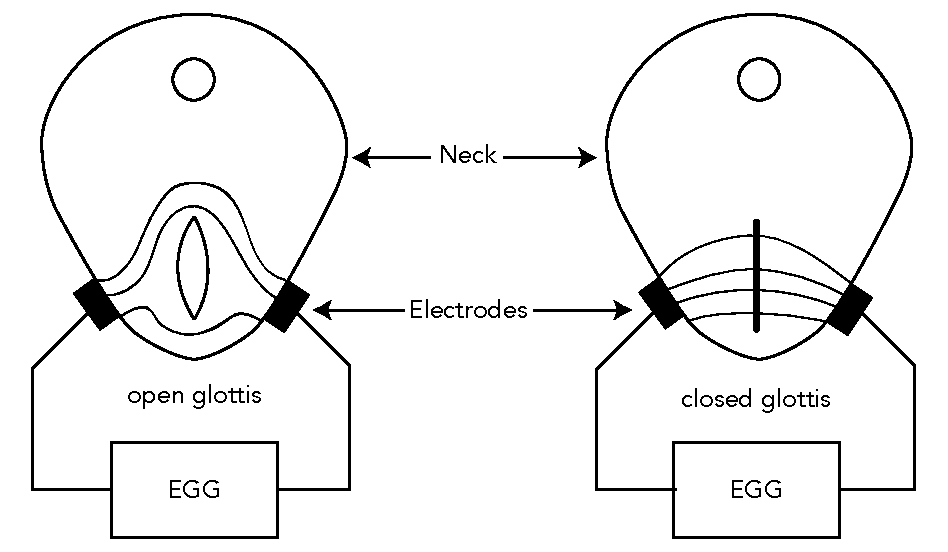
\includegraphics[width=0.80000\textwidth]{../graphics/egg-setup.pdf}
\caption{A schematic representation of the
electroglottograph.\label{f:egg-setup}}
\end{figure}

\section{Methodology}\label{methodology}

\subsection{Equipment setup}\label{s:setup}

\begin{figure}[htbp]
\centering
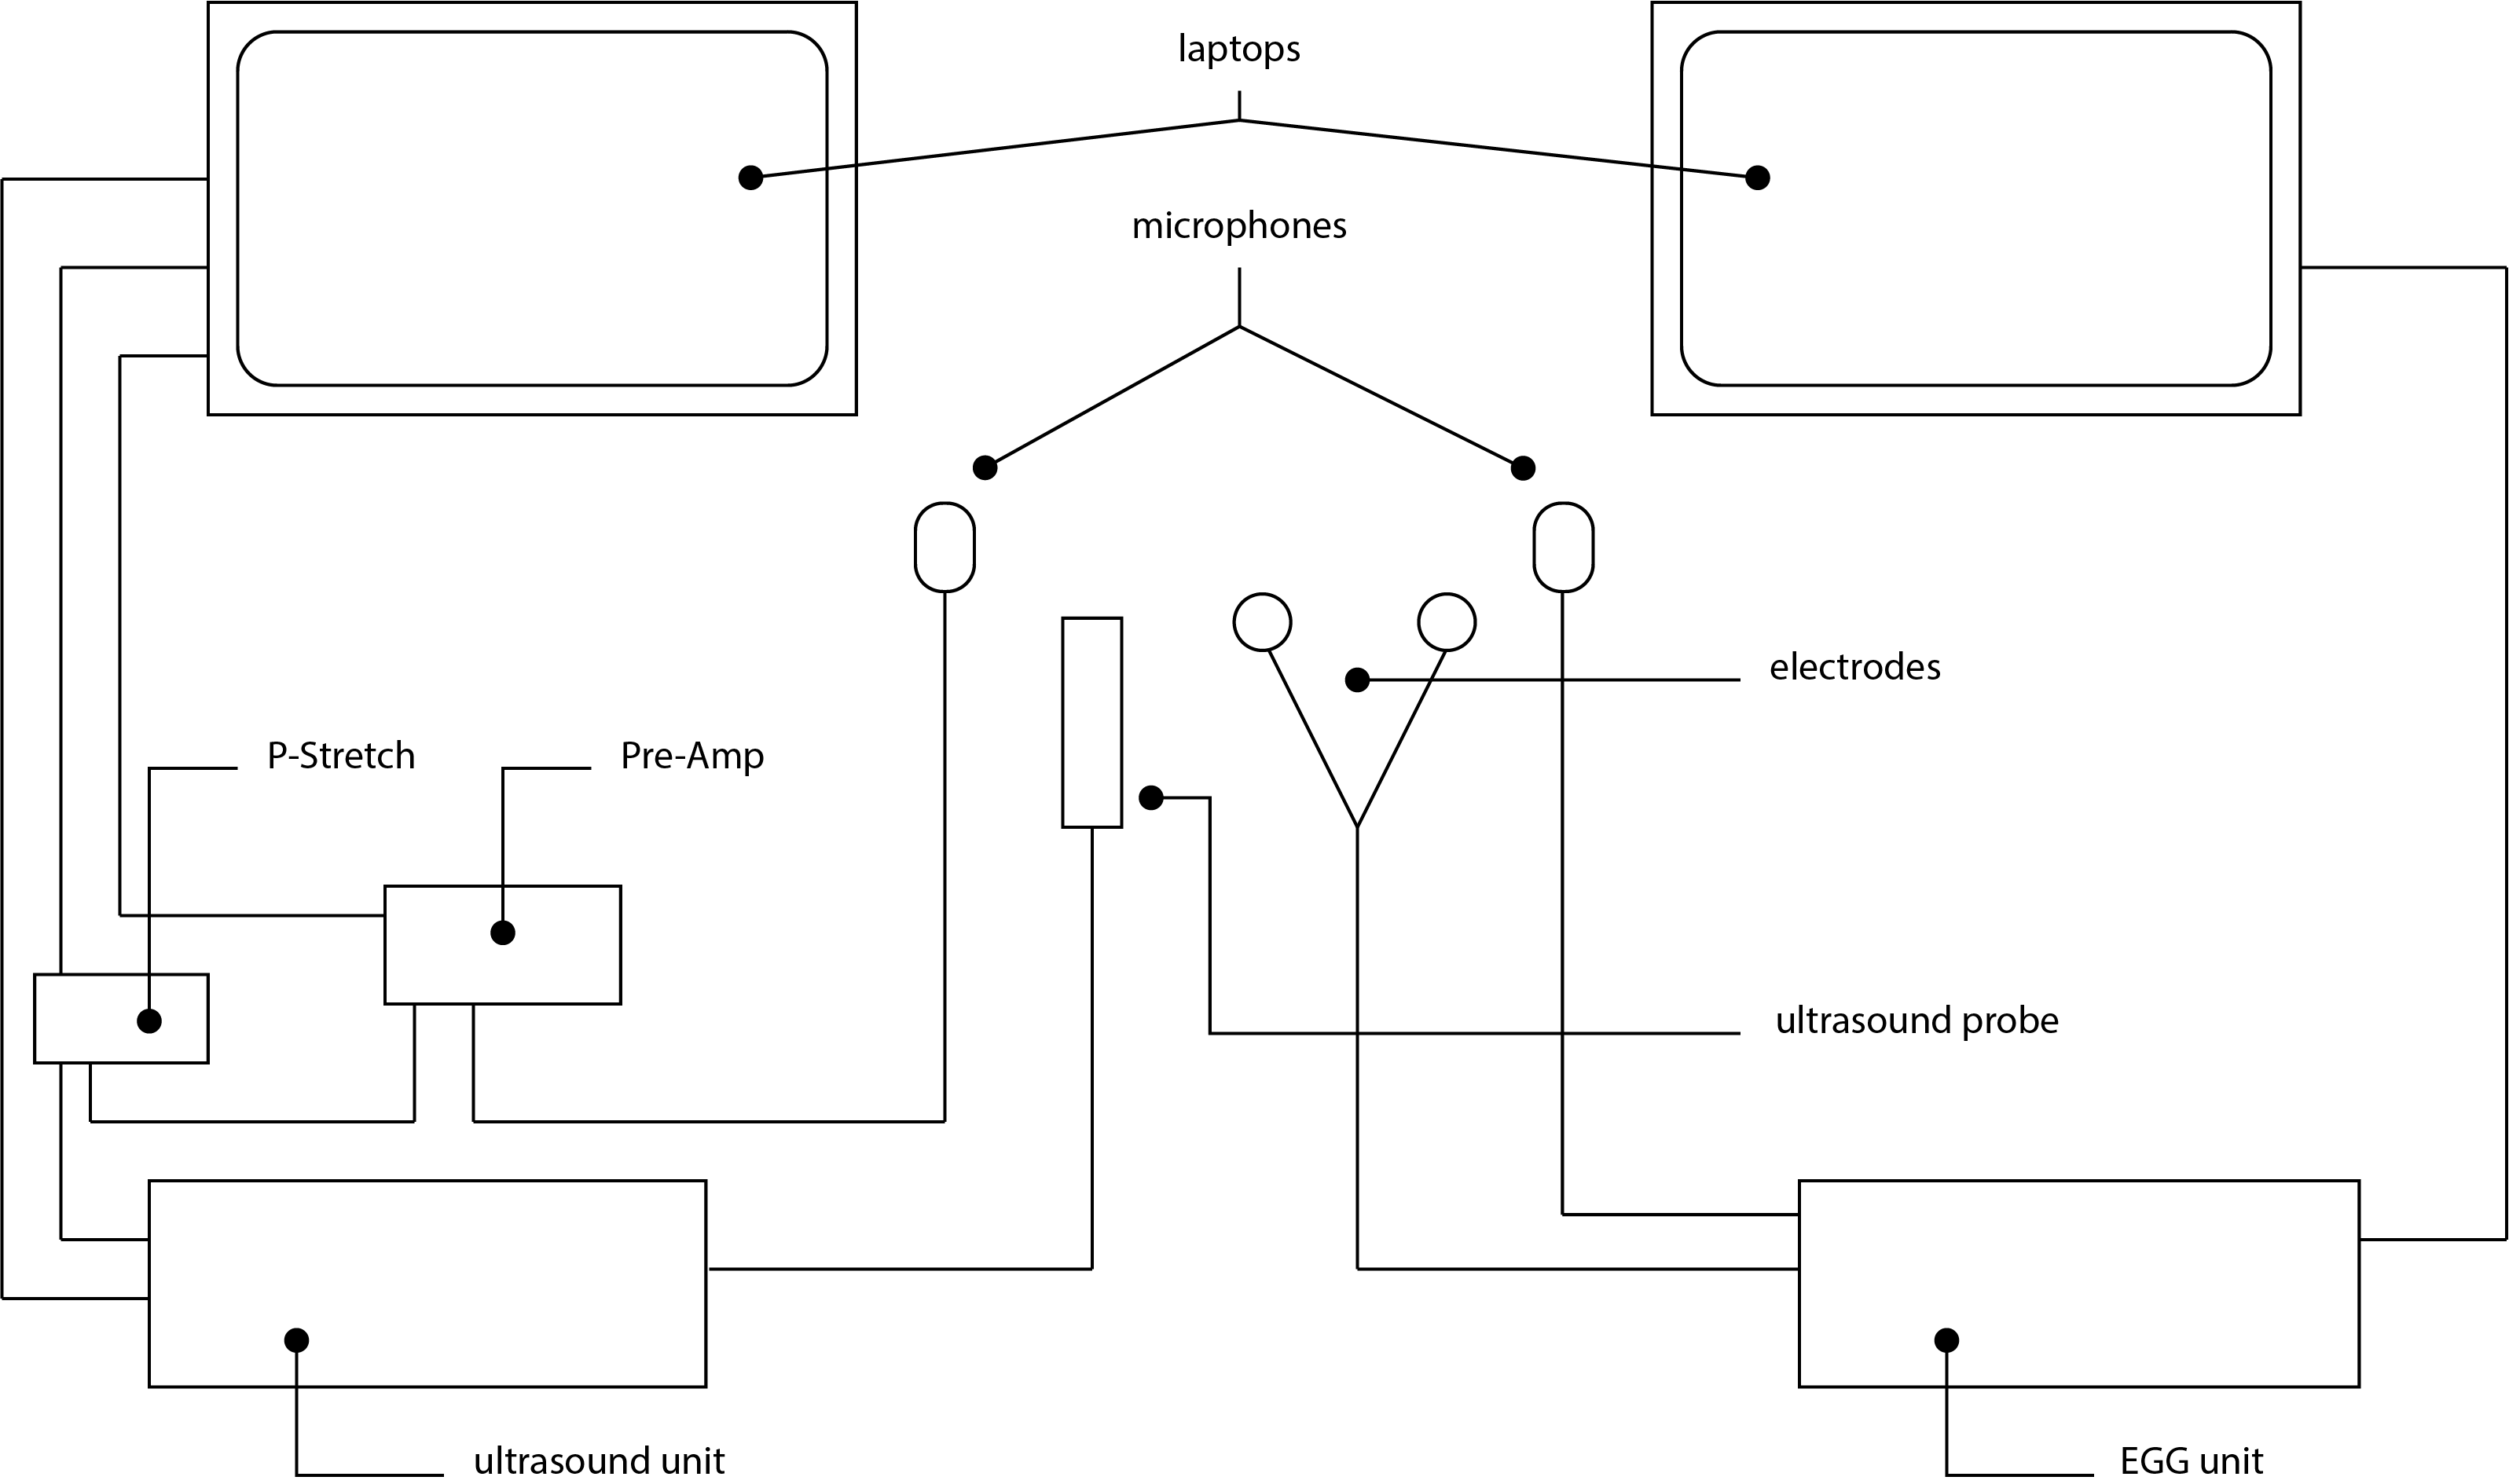
\includegraphics[width=0.80000\textwidth]{../graphics/setup.png}
\caption{Equipment set-up scheme\label{f:setup}}
\end{figure}

\Cref{f:setup} shows the equipment set-up employed. The left part of the
figure shows the ultrasound set-up, while the EGG set-up is shown on the
right. Two separate laptops are used for the acquisition of the
ultrasound and EGG recordings. The ultrasound unit is plugged into one
laptop. A P-Stretch unit (used for signal synchronisation) and the
ultrasound probe are directly connected to the ultrasound unit. The
P-Stretch unit and a microphone feed a pre-amplifier system, which is
plugged into the ultrasound laptop. A second microphone and the
electrodes are connected to the EGG unit, which is plugged into the
second laptop. A TELEMED Echo Blaster 128 system is used for
ultrasonography and a Glottal Enterprises EG2-PCX2 unit for EGG. The
subject wears a headset (a metallic \ldots{}, not shown in
\Cref{f:setup}) which holds the ultrasound probe in position (allowing
free head movement by the subject) and a velcro strap with the EGG
electrodes, located on each side of the thyroid cartilage, at the level
of the glottis. The microphones are clipped to the headset on either
side, at identical height.

\subsection{Acquisition and post-processing of ultrasound and
EGG}\label{acquisition-and-post-processing-of-ultrasound-and-egg}

Ultrasound and EGG inputs are acquired and recorded in separate laptops
by means of, respectively, Articulate Assistant Advanced {[}AAA, {]} and
Praat {[}{]}. Detection of tongue profile and calculation of velocity
measures and consonantal target and release are automatically performed
in AAA using built-in functions. EGG post-processing is described in
\Cref{s:tracegram}.

\subsection{Ultrasound and EGG
synchronisation}\label{ultrasound-and-egg-synchronisation}

Since the signals from the ultrasound machine and the laryngograph are
recorded simultaneously but separately, data from both machines need to
be synchronised after acquisition. Synchronisation is achieved through
the cross-correlation of the audio signals from both sources
\citep{grimaldi2008}. The cross-correlation method creates a new sound
file from two audio files. The created new file is a convolution of the
original files. The time of the maximum amplitude in the convoluted
sound wave is the amount of off-set between the two original files. The
off-set is trimmed from the beginning of the longer audio file, with the
result that the files will be in sync. A measure taken at any particular
time in the ultrasound source can thus be related to a measure taken at
that same time in the laryngograph source.

\subsection{Calculation of dEGG and tracegram
analysis}\label{s:tracegram}

Previous studies have shown that the mathematical first derivative of
the EGG signal helps determine the moments of glottal closure and
opening in each vibration cycle (glottal period). The first derivative
of a signal is basically the velocity of the signal, in other words how
fast the signal changes in time. The time of maximum velocity in the
first derivative of the EGG signal (dEGG) roughly corresponds to the
moment of glottal closure. The time of minimum velocity corresponds to
the moment of glottal opening. Thus, glottal closure and opening for
each glottal period can be extracted from the dEGG.

\citet{herbst2010} describe a new technique, called electroglottographic
wavegram, which displays the variations in the EGG and dEGG signals in a
single graph. A wavegram contains temporal information on the \emph{x}
and \emph{y} axis, while changes in the VFCA are rendered as different
colour intensities on the \emph{z} axis.

The extraction of dEGG maxima and minima has been implemented in this
study using the PRAAT scripting language. The algorithm consists of the
following stages:

\begin{enumerate}
\def\labelenumi{\arabic{enumi}.}
\tightlist
\item
  detection of the glottal periods
\item
  calculation of the dEGG
\item
  extraction of absolute dEGG maximum (dEGG\textsubscript{max}) and
  minimum (dEGG\textsubscript{min}) for each glottal period
\item
  calculation of dEGG\textsubscript{max} and dEGG\textsubscript{min}
  relative to the glottal period
\end{enumerate}

It is conventional to define a glottal period as the time between two
consecutive moments of glottal closure, i.e.~two consecutive dEGG
maxima. However, since the maxima need to be identified in the first
place, an arbitrary definition of glottal period is instead used.
Glottal periods correspond to the intervals between two consecutive EGG
minima {[}cf. \ldots{}{]}. First, the EGG signal is band-pass filtered
(40Hz-10KHz) and smoothing is applied. A weighted sliding-average
smoothing method (triangular smooth) is used, with smooth width \emph{m}
= 11. EGG minima are thus extracted from the smoothed EGG signal. The
interval between any two consecutive minima constitutes a glottal
period.

The dEGG is calculated with the formula \(x_n' = x_{n+1} - x_n\), where
\(x_n\) is the value of the EGG signal at the time n. After calculation,
the resulting dEGG is smoothed with the same method as before
(triangular smooth, \emph{m} = 11). The algorithm then searches for dEGG
maxima and minima within each glottal period (defined as two consecutive
EGG minima). Finally, relative dEGG\textsubscript{max} and
dEGG\textsubscript{min} are calculated as proportions of the respective
glottal period. The resulting values are between 0 (beginning of period)
and 1 (end of period).

As \citet{herbst2010} note, the wavegram technique has the limitation of
not being suitable for quantitative analysis. A new visualisation
technique, based on wavegrams, is introduced here: electroglottographic
tracegram. The tracegram method, even if it reduces the displayed
dimensions, allows a statistical assessment of the varying
dEGG\textsubscript{max} and dEGG\textsubscript{min}, thus constituting a
partial improvement over wavegrams. After the calculation of the
relative dEGG\textsubscript{max} and dEGG\textsubscript{min}, these
values are plotted in a graph on the \emph{y} axis at each time point
which corresponds to the beginning of a glottal period. Since the values
are restricted between 0 and 1 (being proportions), changes in glottal
period (which corresponds to changes in fundamental frequency and hence
pitch) are controlled for. The resulting graph, the tracegram, shows the
traces of dEGG\textsubscript{max} and dEGG\textsubscript{min} as they
change in time, in a way similar to the display of pitch contours.
Statistical analysis is then performed on both traces separately using a
Smoothing Spline ANOVA (SSANOVA).

\section{Statistical testing}\label{statistical-testing}

\section{Pilot study}\label{pilot-study}

I ran a pilot study to verify the performance of the methodology. Two
speakers of Italian (2 males) and two speakers of Polish (1 female, 1
male) were recorded using the setup described in \Cref{s:setup}. The
target words were of the form
C\textsubscript{1}V\textsubscript{1}C\textsubscript{2}V\textsubscript{1},
where C\textsubscript{1} = /p/, V\textsubscript{1} = /a, o, u/,
C\textsubscript{2} = /t, d, k, g/. The words were embedded in
prosodically similar sentences (Italian \emph{Dico X lentamente} `I say
X slowly', and Polish \emph{Mówię X teraz} `I say X now').

\subsection{Results}\label{results}

\begin{figure}[htbp]
\centering
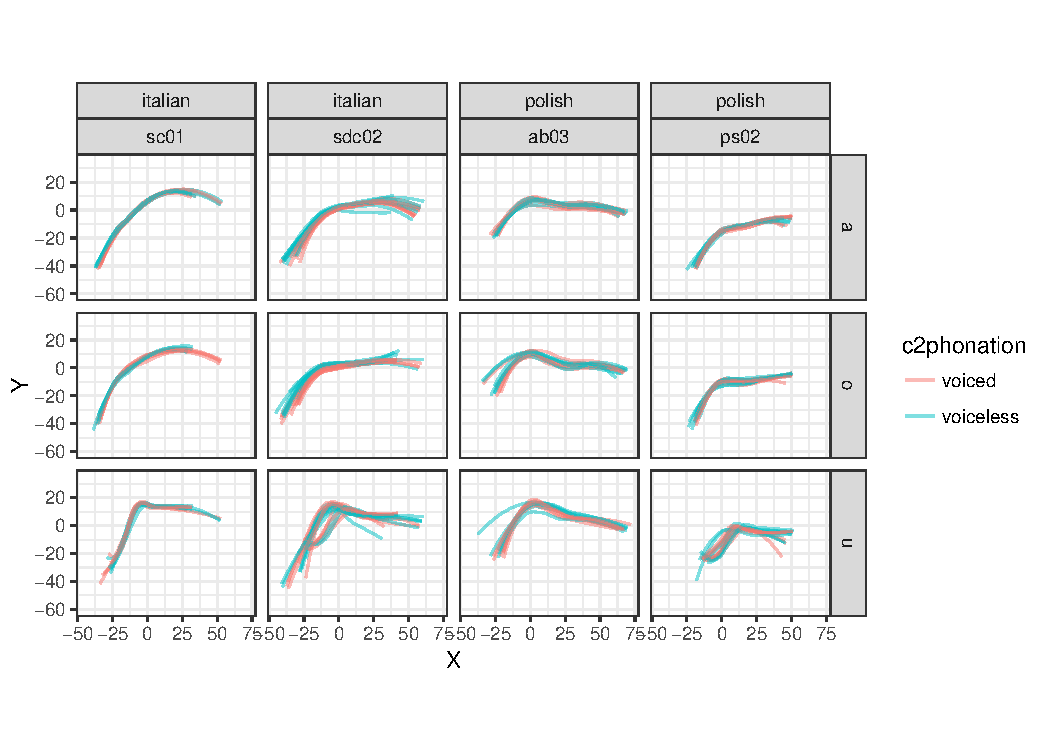
\includegraphics[width=0.90000\textwidth]{../graphics/coronal.pdf}
\caption{Tongue contour at maximum constriction of coronal consonants in
Italian and Polish.\label{f:coronal}}
\end{figure}

\Cref{f:coronal} shows the tongue countours of the speakers of Italian
and Polish. Only the contours at maximum closure of coronal consonants
are plotted, separately for each vowel (rows) and speaker (columns). The
root of the rongue is on the left of each graph, while the tip is on the
right. The contours of the anterior part of the tongue in voiced (red
lines) and voiceless stops (blue lines) overlap both in Italian and
Polish. This indicates that the the saggital shape of the tongue at
maximum constriction is not affected by the voicing of the consonant.
However, the tongue root seems to be advanced in voiced stops (red
lines) compared to voiceless stops (blue lines) in Italian, but not in
Polish. According to a generalised additive mixed effects model fitted
on the Italian and Polish data, the tongue root was significantly
advanced in voiced stops in Italian, while there was no significant
difference in Polish (\Cref{f:it-pl}).

\begin{figure}[htbp]
\centering
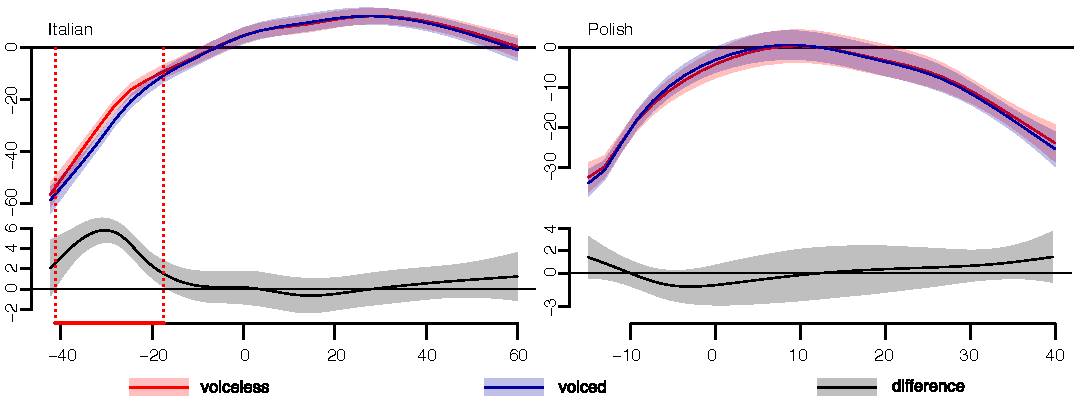
\includegraphics[width=0.90000\textwidth]{../graphics/it-pl.pdf}
\caption{Tongue contour in voiceless and voiced stops at maximum
constriction in Italian (left) and Polish (right). When the confidence
intervals of the difference smooth (grey) do not cross 0 on the y-axis,
they indicate a significant difference (red line on the
x-axis).\label{f:it-pl}}
\end{figure}

The analysis of the EGG data is underway, although, as derived from the
visual inspection of the data, it seems that both Italian and Polish
voiceless stops entail earlier glottal spread, reflected in the
tracegram of these stops, shown in \Cref{f:tracegram}. The dEGG maximum
starts raising at around 60\% of the vowel in Italian and Polish if the
vowel is followed by voiceless stops. A raised dEGG maximum during the
last portion of the vowel indicates that glottal spreading (which is the
configuration of the vocal folds during the production of voiceless
stops) is initiated even before consonant closure is achieved. On the
contrary, there seems to be no significant increase in the dEGG maximum
in voiced stops in neither language.

\begin{figure}[htbp]
\centering
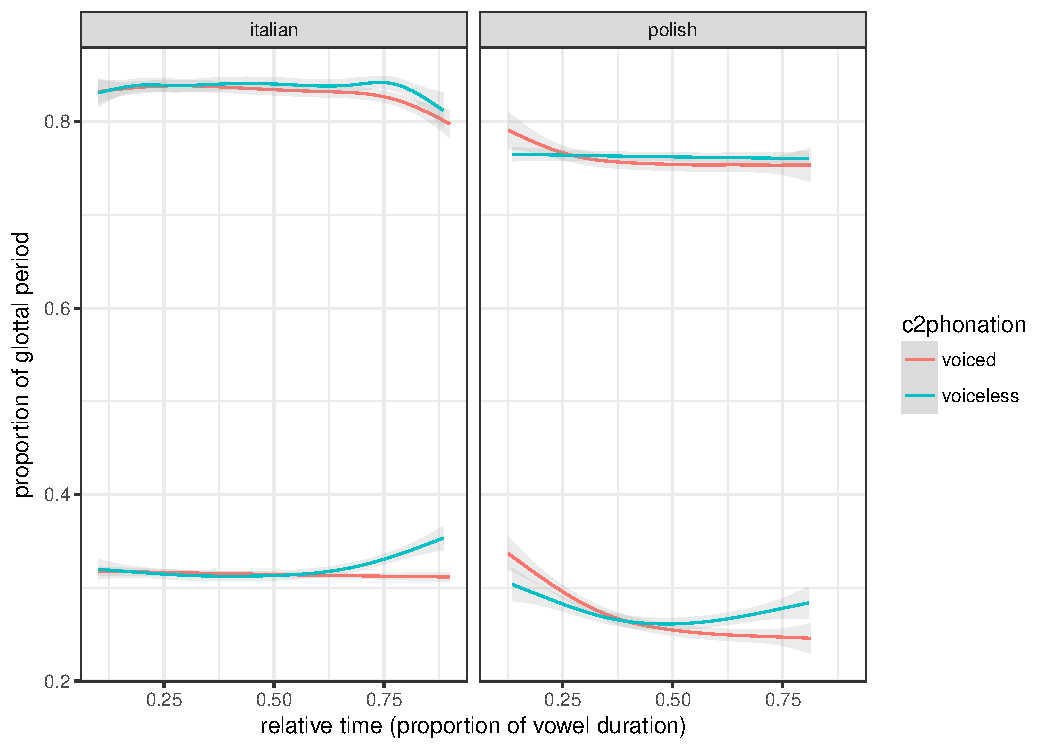
\includegraphics[width=0.80000\textwidth]{../graphics/tracegram.pdf}
\caption{Tracegram.\label{f:tracegram}}
\end{figure}

\renewcommand\refname{References}
\bibliography{linguistics.bib}


\end{document}
